\def\mytitle{ASSIGNMENT} 
\def\myauthor{M Sai Santhosh Kumar}
\def\contact{santhoshmandarapu1221@gmail.com}
\def\mymodule{Future Wireless Communications (FWC)}
\documentclass[journal,12pt]{article}
\usepackage{setspace}
\usepackage{gensymb}
\usepackage{xcolor}
\usepackage{caption}
\usepackage[hyphens,spaces,obeyspaces]{url}
\usepackage[cmex10]{amsmath}
\usepackage{mathtools}
\singlespacing
\usepackage{amsthm}
\usepackage{mathrsfs}
\usepackage{txfonts}
\usepackage{stfloats}
\usepackage{cite}
\usepackage{cases}
\usepackage{subfig}
\usepackage{longtable}
\usepackage{multirow}
\usepackage{graphicx}
\graphicspath{{./images/}}
\usepackage[colorlinks,linkcolor={black},citecolor={blue!80!black},urlcolor={blue!80!black}]{hyperref}
\usepackage[parfill]{parskip}
\usepackage{lmodern}
\usepackage{tikz}
\usepackage{circuitikz}
\usepackage{karnaugh-map}
\usepackage{pgf}
\usepackage[hyphenbreaks]{breakurl}
\usepackage{tabularx}
\usetikzlibrary{calc}
\renewcommand*\familydefault{\sfdefault}
\usepackage{watermark}
\usepackage{lipsum}
\usepackage{xcolor}
\usepackage{listings}
\usepackage{float}
\usepackage{titlesec}
\DeclareMathOperator*{\Res}{Res}
\renewcommand\thesection{\arabic{section}}
\renewcommand\thesubsection{\thesection.\arabic{subsection}}
\renewcommand\thesubsubsection{\thesubsection.\arabic{subsubsection}}

% correct bad hyphenation here
\hyphenation{op-tical net-works semi-conduc-tor}

\titlespacing{\subsection}{1pt}{\parskip}{3pt}
\titlespacing{\subsubsection}{0pt}{\parskip}{-\parskip}
\titlespacing{\paragraph}{0pt}{\parskip}{\parskip}
\newcommand{\figuremacro}[5]{
\begin{figure}[#1]
\centering
\includegraphics[width=#5\columnwidth]{#2}
\caption[#3]{\textbf{#3}#4}
\label{fig:#2}
\end{figure}
}
\lstset{
frame=single, 
breaklines=true,
columns=fullflexible
}
\title{\mytitle}
\author{\myauthor\hspace{1em}\\\contact\\IITH\hspace{0.5em}-\hspace{0.6em}\mymodule}
\date{27-03-2023}
\def\inputGnumericTable{}                
\lstset{
frame=single,
breaklines=true,
columns=fullflexible
}
\begin{document}
\theoremstyle{definition}
\newtheorem{theorem}{Theorem}[section]
\newtheorem{problem}{Problem}
\newtheorem{proposition}{Proposition}[section]
\newtheorem{lemma}{Lemma}[section]
\newtheorem{corollary}[theorem]{Corollary}
\newtheorem{example}{Example}[section]
\newtheorem{definition}{Definition}[section]
\newcommand{\BEQA}{\begin{eqnarray}}
\newcommand{\EEQA}{\end{eqnarray}}
\newcommand{\define}{\stackrel{\triangle}{=}}
\bibliographystyle{article}
\vspace{3cm}
\maketitle
\tableofcontents
\pagebreak
\section{Question}
       Consider a $3$ bit counter,designed using $T$ flip-flops,as shown below:
\begin{figure}[h]
	\centering
        \begin{tikzpicture}
    \draw (2,2) rectangle (5,5);
    \draw (2.75,4) node{$Tp$};
    \draw (4.5,3) node{$P$} -- (5.5,3) -- (6,3);
    \draw (4.5,4) node{$P'$} -- (5.5,4) -- (7,4);
    \draw (7,2) rectangle (10,5);
    \draw (7.75,4) node{$Tq$};
    \draw (9.5,3) node{$Q$} -- (10.5,3) -- (11,3);
    \draw (9.5,4) node{$Q'$} -- (10.5,4) -- (11,4);
    \draw (12,2) rectangle (15,5);
    \draw (12.75,4) node{$Tr$};
    \draw (14.5,3) node{$R$} -- (15.5,3) -- (16,3);
    \draw (14.5,4) node{$R'$} -- (15.5,4) -- (15,4);
    \draw (0,0) node[above]{$clock$}  -- (13.5,0);
    \draw (2.75,0) -- (2.75,2);
    \draw (7.75,0) -- (7.75,2);
    \draw (12.75,0) -- (12.75,2);
    \draw (9.5,4) -- (12.75,4); 
    \draw (16,3) -- (16,6); 
    \draw (16,6) -- (0,6);  
    \draw (0,6) -- (0,4);
    \draw (0,4) -- (2.75,4);
\end{tikzpicture}

        \caption{}
        \label{figs:tflipflop.}
\end{figure}	
       Assuming the initial state of the counter given by $PQR$ as $000$, what are the next three states?
\section{Components}
\begin{table}[h]
\centering
\begin{tabular}{|c|c|c|}
\hline
	\textbf{Component}& \textbf{values} & \textbf{Qantity}\\
\hline
	Arduino & UNO & 1 \\
\hline
	Jumperwires & M-M & 35 \\
\hline
	Breadboard & & 2 \\
\hline
	LED & & 3\\
\hline
	Resistor & 220ohms & 3 \\
\hline
	IC & 7476 & 3 \\
\hline
\end{tabular}
\end{table}
\begin{center}
Figure.a
\end{center}
\section{TruthTable}
\centering
\begin{tabularx}{0.46\textwidth} {
                | >{\centering\arraybackslash}X
                | >{\centering\arraybackslash}X
                | >{\centering\arraybackslash}X
                | >{\centering\arraybackslash}X | }
\hline
\textbf{T} & \textbf{Q} & \textbf{Q'}\\
\hline
0 & Q & Q' \\
\hline
1 & Q' & Q \\
\hline
\end{tabularx}
\begin{center}
Truth table for "T" flipflop	
\end{center} 
\section{ExcitationTable}
\centering
  \begin{tabularx}{0.46\textwidth} {
  | >{\centering\arraybackslash}X
  | >{\centering\arraybackslash}X
  | >{\centering\arraybackslash}X
  | >{\centering\arraybackslash}X
  | >{\centering\arraybackslash}X
  | >{\centering\arraybackslash}X | }
\hline
\textbf{Q} & \textbf{Qn} & \textbf{T}\\
\hline
0 & 0 & 0 \\
\hline
0 & 1 & 1 \\
\hline
1 & 0 & 1 \\
\hline
1 & 1 & 0 \\
\hline
\end{tabularx}
\begin{center}
Excitation table of T- flipflop
\end{center}
\section{Truthtable(3-stages)}
  \begin{table}[h]
  \centering
  \begin{tabular}{|c|c|c|c|c|c|}
  \hline
  \textbf{P} & \textbf{Q} & \textbf{R} & \textbf{P+} & \textbf{Q+} & \textbf{R+} \\
 \hline
 0 & 0 & 0 & 0 & 1 & 1 \\
 \hline
 0 & 1 & 1 & 1 & 0 & 1 \\
\hline
 1 & 0 & 1 & 0 & 0 & 0 \\
\hline
\end{tabular}
\end{table}
\begin{center}
Figure :b
\end{center}
\pagebreak
\section{3stages}
\begin{figure}[ih]
	\centering
	\input{figures/fig2.tex}
	\caption{}
	\label{fig:2.}
\end{figure}
\begin{figure}[ih]
        \centering
        \input{figures/fig3.tex}
        \caption{}
        \label{fig:3.}
\end{figure}
\begin{figure}[ih]
        \centering
        \input{figures/fig4.tex}
        \caption{}
        \label{fig:4.}
\end{figure}
\vspace{5mm}
\newpage
\section{Hardware}
        The 7476 is a master—slave J-K and the 74LS76 is a negative edge-triggered J-K flip-flop. Both chips have the same pin configuration. Below is the pin diagram of IC7476. \\
\begin{figure}[ih]
	\centering
	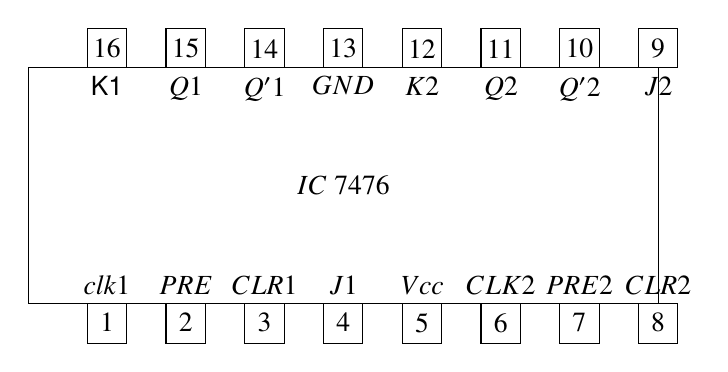
\begin{tikzpicture}
    \draw (0,2) rectangle (8,5);
    \draw (4,3.5) node{$IC$ $7476$};
    \draw (0.75,2) rectangle(1.25,1.5);
    \draw (1,2) node[below]{$1$};
    \draw (1,2) node[above]{$clk1$};
    \draw (1.75,2) rectangle (2.25,1.5);
    \draw (2,2) node[below]{$2$};
    \draw (2,2) node[above]{$PRE$};
    \draw (2.75,2) rectangle (3.25,1.5);
    \draw (3,2) node[below]{$3$};
    \draw (3,2) node[above]{$CLR1$};
    \draw (3.75,2) rectangle (4.25,1.5);
    \draw (4,2) node[below]{$4$};
    \draw (4,2) node[above]{$J1$};
    \draw (4.75,2) rectangle (5.25,1.5);
    \draw (5,2) node[below]{$5$};
    \draw (5,2) node[above]{$Vcc$};
    \draw (5.75,2) rectangle (6.25,1.5);
    \draw (6,2) node[below]{$6$};
    \draw (6,2) node[above]{$CLK2$};
    \draw (6.75,2) rectangle (7.25,1.5);
    \draw (7,2) node[below]{$7$};
    \draw (7,2) node[above]{$PRE2$};
    \draw (7.75,2) rectangle (8.25,1.5);
    \draw (8,2) node[below]{$8$};
    \draw (8,2) node[above]{$CLR2$};
    \draw (0.75,5) rectangle (1.25,5.5);
    \draw (1,5) node[above]{$16$};
    \draw (1,5) node[below]{K1};
    \draw (1.75,5) rectangle (2.25,5.5);
    \draw (2,5) node[above]{$15$};
    \draw (2,5) node[below]{$Q1$};
    \draw (2.75,5) rectangle (3.25,5.5);
    \draw (3,5) node[above]{$14$};
    \draw (3,5) node[below]{$Q'1$};
    \draw (3.75,5) rectangle (4.25,5.5);
    \draw (4,5) node[above]{$13$};
    \draw (4,5) node[below]{$GND$};
    \draw (4.75,5) rectangle (5.25,5.5);
    \draw (5,5) node[above]{$12$};
    \draw (5,5) node[below]{$K2$};
    \draw (5.75,5) rectangle (6.25,5.5);
    \draw (6,5) node[above]{$11$};
    \draw (6,5) node[below]{$Q2$};
    \draw (6.75,5) rectangle (7.25,5.5);
    \draw (7,5) node[above]{$10$};
    \draw (7,5) node[below]{$Q'2$};
    \draw (7.75,5) rectangle (8.25,5.5);
    \draw (8,5) node[above]{$9$};
    \draw (8,5) node[below]{$J2$};
\end{tikzpicture}

	\caption{}
	\label{pindiagram.}
\end{figure}
\section{Implementation}
The connections between Arduino UNO and three IC 7476 is given in below Table \\
\begin{table}[h]
	\begin{center}
	\begin{tabular}{|c|c|c|c|c|c|c|c|c|c|c|}
		\hline & \multicolumn{3}{|c|}{INPUT} & \multicolumn{3}{|c|}{OUTPUT} & CLOCK & Vcc & GND \\
		\hline ARDUINO & D2 & D3 & D4 & D5 & D6 & D7 & 13 & 5V & GND \\
		\hline 7476 & \multicolumn{3}{|c|}{16} & \multicolumn{3}{|c|}{15} & 1 & 5 & 13 \\
		\hline
	\end{tabular}
	\end{center}
	\caption{connections}
	\label{table:1}
\end{table}
\section{Procedure}
\begin{raggedright}
    1.Connect the circuit as per the above tble.\\
    2.connect the output pins to the LED's \\
    3.Connect inputs to Vcc for logic 1,ground for logic 0 \\
    4.Execute the circuit using the below code.\\
\begin{table}[h]
\centering
	\begin{tabular}{|c|}
	\hline
	https://github.com/santhosh-1221/ \\
		ide/blob/main/code/segment.cpp \\
	\hline
\end{tabular}
\end{table}
     5.Change the values of Q1,Q2,Q3 in the code and verify the truth table \\
\end{raggedright}
\bibliographystyle{article}
\end{document}

